\documentclass[sigconf]{acmart}

\usepackage{booktabs}
\usepackage[brazil]{babel}   
\usepackage[utf8]{inputenc}
\usepackage[]{algorithm2e}
\usepackage{graphics}
\usepackage{fancyhdr}


% Copyright
%\setcopyright{none}
%\setcopyright{acmcopyright}
%\setcopyright{acmlicensed}
\setcopyright{rightsretained}
%\setcopyright{usgov}
%\setcopyright{usgovmixed}
%\setcopyright{cagov}
%\setcopyright{cagovmixed}

% DOI
%\acmDOI{10.475/123_4}

% ISBN
%\acmISBN{123-4567-24-567/08/06}

%Conference
\acmConference[Pesquisa Operacional]{Trabalho Final da disciplina de
Pesquisa Operacional da UFF, 2018.2}
\acmYear{2018}
\copyrightyear{2018}

%\acmArticle{4}
%\acmPrice{15.00}

\begin{document}
\title{Proposta de solução do Problema de Dominação de Rainhas Utilizando ILS}
\titlenote{Produces the permission block, and copyright information}

\author{Maria Edoarda Vallim Fonseca}
\affiliation{%
  \institution{Institute of Computing -- UFF}
  \city{Niterói}
  \country{Brazil}
}
\email{medoarda@id.uff.br}

\author{Thales Athayde Santos}
\affiliation{%
  \institution{Institute of Computing -- UFF}
  \city{Niterói}  
  \country{Brazil}
}
\email{thalesathaydesantos@id.uff.br}

\begin{abstract}
In this paper, we propose a solution to the Dominating Queens Problem
using Iterative Local Search and compare our results with a previous 
solution using Genetic Algorithm.
\end{abstract}

%
% The code below should be generated by the tool at
% http://dl.acm.org/ccs.cfm
% Please copy and paste the code instead of the example below.
%

\keywords{Dominating Queen Problem, ILS, Metaheuristic}

\maketitle

%%%%%%%%%%%%%%%%%%%%%%%%%%%%%%%%%%%%%%%%%%%%%%%%%%%%%%%%%%%%%%%%%%%%%%
\section{Introdução}

O problema de dominação de rainhas é muito bem conhecido
dentre os problemas de xadrez. Nele, dado um tabuleiro \textit{nxn}, temos n quadrados dispostos nas linhas e n quadrados nas colunas. Quando uma rainha Q é disposta no tabuleiro, ela domina a linha, a coluna, e as diagonais que passam pela sua posição. O objetivo do problema é descobrir a disposição da menor quantidade de rainhas possível de forma à dominar todo o tabuleiro.

 Muitos pesquisadores focaram em descobrir os limites superior e inferior do problema desde a década de 70,  e o número mínimo possível de rainhas para solucionar o problema ($\gamma(\textbf{Qn})$) foi calculado para diversos tamanhos de tabuleiro (vide tabela~\ref{tabela1})~\cite{art3,art43,art44,art45}.

 Algoritmos evolucionários provaram ter sucesso para resolver e otimizar uma grande variedade de problemas complexos, incluindo problemas combinatórios, como o estudado aqui, em um tempo computacional razoavelmente aceitável.~\cite{doerr2011evolutionary}

\textit{Local Search}, ou Busca Local, é um método heurístico para resolver problemas computacionalmente difíceis. Busca local pode ser usada em problemas que possam ser formulados como achar a solução maximizando um critério entre várias soluções possíveis. Algoritmos de busca local movem de solução à solução no espaço de soluções possíveis aplicando mudanças locais, até uma solução dita ótima ser encontrada.~\cite{hoos2004stochastic}

Um dos problemas da Busca Local é que ela pode ficar presa em um mínimo local, sem conseguir melhorar seu resultado. Para contornar esse problema, utiliza-se \textit{Iterative Local Search}, ou Busca Local Iterativa. Essa modificação consiste em iterar sobre chamadas da busca local, cada vez começando de um ponto diferente do conjunto de solução perturbando o mínimo local atual de modo que faça a solução chegar em outro ótimo local. Esta perturbação não pode ser muito forte nem muito fraca, pois corre o risco dela acabar encontrando o mesmo mínimo local ou servir como uma inicialização aleatória.~\cite{lourencco2010iterated}

  Neste artigo, propomos uma solução baseada em \textit{Iterative Local Search} para o Problema de Dominação de Rainhas. Nossos resultados serão comparados diretamente com o método descrito em~\cite{alharbi2017genetic}, que utiliza Algoritmo Genético e é o mais comumente encontrado para solucionar este problema. Depois disso, iremos debater os resultados alcançados.

\begin{table*}[ht]
  \caption{Número mínimo de rainhas para dominação total $\gamma(\textbf{Qn})$ de um tabuleiro de tamanho $\textit{n}$.}
  \begin{tabular}{l*{18}{c}r}
    n              & 1 & 2 & 3 & 4 & 5  & 6 & 7 & 8 & 9 & 10 & 11 & 12 & 13 & 14 & 15 & 16 & 17 & 18 \\
    \hline
    $\gamma(\textbf{Qn})$ & 1 & 1 & 1 & 3 & 3 & 4 & 4 & 5 & 5 & 5 & 5 & 7 & 7 & ~$\leq$8 & $\leq$9 & $\leq$9  & 9 & 9 \\
  \end{tabular}
  \label{tabela1}
\end{table*}


%Tabela \ref{tabela1}: Número mínimo de rainhas para dominação total de um tabuleiro de tamanho $\textit{n}$.

%%%%%%%%%%%%%%%%%%%%%%%%%%%%%%%%%%%%%%%%%%%%%%%%%%%%%%%%%%%%%%%%%%%%%%
\section{Motivação}

Decidimos escolher o \textit{Dominating Queens Problem} por ter sido um dos temas abordados por um dos membros do grupo durante as apresentações de trabalho da disciplina, o que nos deu um certo grau de familiaridade com o assunto. Pesquisando mais à fundo, vimos que as soluções mais comuns para a solução do Problema de Dominação de Rainhas eram com \textit{Backtracking} e Algoritmo Genético. Além disso, de acordo com~\cite{alharbi2017genetic}, existem muitos artigos procurando os limites superior e inferior do problema, mas não existe muito esforço de pesquisa
na busca de soluções práticas para o problema.

Visto essa situação, decidimos propor uma solução baseada em \textit{Iterative Local Search} para o problema e comparar os resultados com uma solução em Algoritmo Guloso.

%%%%%%%%%%%%%%%%%%%%%%%%%%%%%%%%%%%%%%%%%%%%%%%%%%%%%%%%%%%%%%%%%%%%%%
\section{Trabalhos Relacionados}

\begin{figure}
  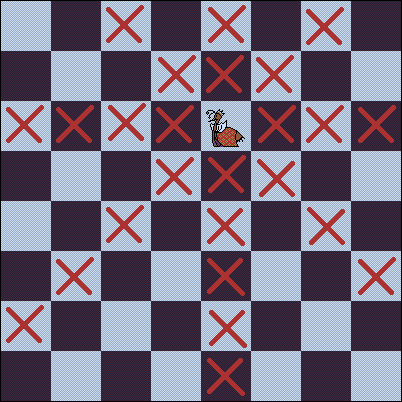
\includegraphics[width=\linewidth]{dom1rainha8x8.png}
  \caption{Exemplo da linha de dominação de uma rainha em um tabuleiro de xadrez \textit{8x8}}
  \label{fig:1rainha}
\end{figure}

Figure \ref{fig:1rainha} mostra a dominação de uma rainha em um tabuleiro \textit{8x8}.

\begin{figure}
  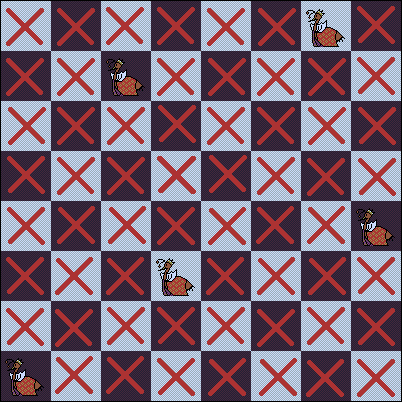
\includegraphics[width=\linewidth]{dom2rainha8x8.png}
  \caption{Exemplo de um tabuleiro de tamanho \textit{8x8} sendo completamente dominado por
  quatro rainhas}
  \label{fig:2rainha}
\end{figure}

Figure \ref{fig:2rainha} shows a sdfsdfwererWboat.

Um problema semelhante, proposto em 1850, conhecido como problema das n-rainhas teve muitos esforços focados nele para sua solução. O problema das n-rainhas é descrito como: dado um tabuleiro nxn, qual seria a disposição das rainhas de modo que nenhuma rainha consiga atacar a outra. Houve muita pesquisa em torno deste problema, e suas soluções utilizam desde teoria matemática até teoria dos grafos. O estudo desse tipo de problema pode beneficiar várias áreas como controle de tráfego, prevenção de \textit{deadlocks} e armazenamento de memória paralela.~\cite{bell2009survey}


%%%%%%%%%%%%%%%%%%%%%%%%%%%%%%%%%%%%%%%%%%%%%%%%%%%%%%%%%%%%%%%%%%%%%%
\section{Methodology}

O \textit{Local Search} foi implementado com 1 de distância pela nossa implementação estar utilizando uma matriz e não um vetor contendo todas as posições do tabuleiro. Embora usar um \textit{Local Search} com distâncias maiores gere resultados melhores, isso teria a consequência negativa de aumentar exponencialmente o tempo computacional da execução do algoritmo.

Pseudocódigo do ILS
\begin{algorithm}
  \KwData{rainhas, tabuleiro}
  \KwResult{how to write algorithm with \LaTeX2e }
  initialization\;
  listaMovimentos = [0..7]\;
  melhorResultado\;
  \While{rainhas}{
  
   embaralha(rainhas)\;
   \eIf{understand}{
    go to next section\;
    current section becomes this one\;
    }{
    go back to the beginning of current section\;
   }
  }
  \caption{Pseudocódigo do algoritmo de ILS utilizado}
 \end{algorithm}

 \begin{algorithm}
  \KwData{rainhas, tabuleiro}
  \KwResult{how to write algorithm with \LaTeX2e }
  initialization\;
  listaMovimentos = [0..7]\;
  melhorResultado\;
  \While{rainhas}{
  
   embaralha(rainhas)\;
   \eIf{understand}{
    go to next section\;
    current section becomes this one\;
    }{
    go back to the beginning of current section\;
   }
  }
  \caption{Pseudocódigo do Algoritmo Genético utilizado}
 \end{algorithm}
 

%%%%%%%%%%%%%%%%%%%%%%%%%%%%%%%%%%%%%%%%%%%%%%%%%%%%%%%%%%%%%%%%%%%%%%
\section{Resultados}

Nossos testes foram rodados em uma máquina Intel Core i5-7200U com 8GB de RAM, usando o sistema operacional Manjaro Linux com o pacote gráfico KDE Plasma. A linguagem de programação utilizada foi Python 3.7.1.

%%%%%%%%%%%%%%%%%%%%%%%%%%%%%%%%%%%%%%%%%%%%%%%%%%%%%%%%%%%%%%%%%%%%%%
\section{Conclusão}

Text...

\bibliographystyle{ACM-Reference-Format}
\bibliography{bibliography}

\end{document}
